% 1.	Introduction (cadre général) / Introduction (general framework): 1 page

\hspace*{0.3cm}

% 1.	Introduction (cadre général) / Introduction (general framework): 1 page

\hspace*{0.3cm}
\color{red}  ALMOST FINAL DRAFT  \color{black}
\subsection{Introduction}
This thesis project focuses on the development and implementation of Markov Chain Monte Carlo (MCMC) techniques, as well as their multi-level and multi-index extensions (MLMCMC and MIMCMC respectively) techniques for Bayesian inverse problems (BIP) arising in seismic
and geophysical applications; such as seismic inversion and earthquake
source estimation. The goal of these type of problems is to determine a set of parameters $\te$, which identify e.g, the earthquake source characteristics, based on few recorded waveforms at the surface. We will use the elasto-dynamic wave  equation to model such seismic event, and will take the recorded waveform to be the time series of the ground displacement\footnote{We remark however that in practice these receiver can also measure  other wave related quantities, such as velocity or acceleration of the ground at the recording position. } at different receivers scattered throughout the surface. In this case, we take the set of unknown parameters $\te$ to be properties related to the source function (location, set-off time, moment tensor), as well as the material properties of the medium, such as density and Lam\'e parameters.  Traditionally, seismic inversion has been performed using a deterministic approach, by introducing a cost functional $J(\te)$ measuring the misfit between the modeled surface waveforms and the observed ones. This cost functional is then minimized using traditional optimization algorithm to find a minimizer (see, e.g, \cite{tromp2005seismic,burstedde2009algorithmic}). In statistical terms, this approach can often be interpreted as a maximum likelihood point estimation. However, there is a growing need to quantify the uncertainty in these methods \cite{SRCMOD}, by adopting, for instance, a Bayesian approach and sampling techniques such as MCMC. The aim of this work is to develop accelerated and efficient MCMC algorithms to tackle this problem.
\subsection{Objectives}
Modern computing facilities and computational techniques are starting to make Bayesian inversion approaches and  MCMC feasible for large scale inverse problems involving partial differential equations (PDEs) \cite{stuart2010inverse}.There is a wealth of literature devoted to those problem arising from elliptic PDEs (see, for example\cite{stuart2010inverse}), however, this is otherwise rather scarce for hyperbolic equations. One of the first objectives from this work is then to extend the BIP theory to cover these type of problems. An additional issue with a MCMC computation is its inherent cost. Contrary to plain Monte Carlo, MCMC is sequential in nature and produces samples that are, in general, correlated. One proposed idea to mitigate this burden is the use of multi-level  samplers \cite{dodwell2015hierarchical,hoang2013complexity,giles2008multilevel}, for which most of the work is done using a coarse discretization of the PDE, and the sample thus obtained is then ``corrected'' using more refined discretization levels. there are few results available so far. This is a rather new approach to MCMC techniques and as such, there are rather few results available so far. A further improvement on the multi-level sampler is offered by the multi-index technique \cite{haji2016multi} there are the multi-index samplers, for which the computational cost can be reduced even further \color{red} by taking different discretization directions. \color{black}.
% In summary, this thesis will cover the following topics, some of which have already been explored and are currently the topic of an upcoming paper (in draft state as of \today). 
%\begin{enumerate}
%	\item Formulation of the BIP and study of its well-possedness for the hyperbolic case.
%	\item Implementation of efficient and addaptive MLMCMC schemes.
%	\item Implementation of efficient and addaptive MIMCMC schemes.
%\end{enumerate}
%and their validation with some well defined case studies in 2 and 3 dimensions. 
\subsection{Problem Set-up}
We are interested in determining  the earthquake properties of a seismic event. Experimentally,  data  $\mathbf{y}\in \R^d$, assumed to be  polluted by some additive random noise $\eta$, is recorded at $N_r$ receivers and at $N_t$ time instances. This receivers can be located, for example, at the surface of the earth or in observation wells.  The recorded data can be described by an observation operator $\mathcal{F}$  applied to a realization of a model for the seismic wave propagation, $\uu:=\uu(\te)$, viewed as a map from a parameter space $\Omega$ to $\R^d$. Based on this, our aim is then to  determine a conditional probability distribution $\pi(\te|y)$  of a set of parameters $\theta\in \Omega$ such that  $\mathcal{F}(\te)=\mathcal{F}(\uu(\te))$ closely resembles the measured data $\bm{y}$.  In the following subsections we will describe in more detail the model used to describe the seismic motion, the observation operator, and the Bayesian inversion procedure used to obtain $\pi(\te|y)$.
\begin{figure}
	\centering
	\includegraphics[width=0.5\linewidth]{setup}
	\caption{Experimental setup of the problem. An earthquake generated at source travels through material properties and the displacement of the earth is recorded at the receivers (purple squares). Based on the recording data of the receivers, we employ MCMC techniques to recover the source location. }
	\label{fig:setup}
\end{figure}

\subsubsection{Forward Problem}

We follow the analysis presented  in \cite{ motamed2013stochastic, motamed2015analysis,kocher2014variational,joly2003variational}. We denote the spatial variable by $\xx$ and the set of unknown parameters by $\te$. Consider an elastic,  non-homogeneous medium in an open, bounded set  $D\subset \R^d$, with $\partial D=\Gamma_D\cup \Gamma_N$, $\Gamma_D\cap \Gamma_N=\emptyset$, $|\Gamma_D|,\ |\Gamma_N|>0$, for $d=2,3$ and a time interval $I=[0,T]$. Given some complete probability space $(\Omega,F,P)$, \color{red} where $\Omega$ is...\color{black} we can pose the following stochastic initial boundary value problem given by \begin{subequations}\label{strongform}
	\begin{align}
	&\varrho(\xx,\te)\uu_{tt}(t,\xx,\te)-\del\cdot\mathbf{\sig}(\uu(t,\xx,\te))=\ff(t,\xx,\te) & \text{in } I\times D\times \Omega\\
	&\uu(0,\xx,\te)=\mathbf{g_1}(\xx), \ \ \uu_t(0,x,\te)=\mathbf{g}_2(\xx) & \text{on } \times D\times \Omega\\
	&\sig(\uu(t,\xx,\te))\cdot\mathbf{n}=\mathbf{0}& \text{on }I\times\Gamma_N\times \Omega,\\
	&\uu(t,\xx,\te)=\bm{0}&\text{ on } I\times\Gamma_D\times \Omega,
	\end{align}
\end{subequations}
where  $\uu: I\times D\times\Omega  \rightarrow\R^d$ $,\xx\in \R^d,\te\in\Omega, t\in I$, and with  $\sig=\lambda(\xx,\te)\del\cdot\uu I +\mu(\xx,\te)(\del\uu+(\del\uu)^T)$. Here we denote by $\uu$  the displacement vector, by $\varrho>0$ the material density, by $\lambda,\mu$ the Lam\'e parameters,  and by $\ff$ a (generalized) body force. \begin{assumption}\label{as:th} \color{red} include comment on assumptions\color{black}
	Let $s\geq 0$ be an integer. We assume that \begin{eqnarray}
	\ff(\cdot,\cdot,\te)\in\LL^2([0,T];\HH^s(D))\text{ for a.e. $\te\in \Omega$}, & \mathbf{g}_1\in \HH^{s+1}(D), &\mathbf{g}_2\in \mathbf{H}^s(D), \ \ s\geq 0.
	\end{eqnarray}
\end{assumption}
\noindent Under Assumption \ref{as:th}, problem (\ref{strongform}) admits a unique solution for a.e $\te \in \Omega$. We can then interpret the solution $\uu(t,\xx,\te)$ as a Banach space-valued function on $\Omega$  \cite{motamed2015analysis}, \begin{equation}\label{eq:wf_s}
\uu=\uu(\te):\Omega\rightarrow\bf{V}:=\mathbf{C}^0([0,T];\HH^{s+1}(D))\cap\mathbf{C}^1([0,T];\HH^s(D))\cap\HH^{2}([0,T];\HH^{s-1}(D)), \ \ s\geq 0.
\end{equation}
In turn, (\ref{eq:wf_s}) is a weak solution to problem (\ref{strongform}) provided that at $t=0$, $\uu(\te)=\mathbf{g}_1,\ \uu_t(\te)=\mathbf{g}_2$ and that for all test functions $\vv\in \mathbf{C}_0^\infty([0,T];H^1(D))$ the following weak formulation holds \begin{eqnarray}
\int_0^T\int_{D}\left(\varrho \uu_{tt}\cdot\vv+\del\vv:\sig(\uu)\right)d\xx dt=\int_0^T\int_{ D}\ff\cdot\vv d\xx dt.
\end{eqnarray}
For the analysis of the well possedness of the Bayesian inverse problem we will need $\uu$ to be Lipschitz in $\Omega$. To this end, we \color{red} quote,recall,...\color{black} the following theorem, presented in \cite{motamed2015analysis}:
\begin{theorem}\label{thm:lips} For the solution of problem (\ref{strongform}) with data given by Assumption \ref{as:th}  \color{red} check on additional assumptions on Motamed's paper \color{black} and with uniformly elliptic material properties,  we have that
	\begin{equation}
	\partial_{\theta_n}\uu(\te)\in\mathbf{C}^0([0,T];\HH^{s}(D)), \ \ s\geq 0,
	\end{equation}
	where $\theta_n$ denotes the $n^\text{th}$ component of $\te$. Moreover, $	\partial_{\theta_n}\uu(\te)$ is uniformly bounded in $\Omega$.
\end{theorem}
\begin{proof}
	The previous theorem is a particular case of Theorem 3 in \cite{motamed2015analysis}, for the case $k=1, $  \color{red} what is k?\color{black}and $s\geq 0$. 
\end{proof}
\begin{corollary}
	Under the assumptions of the previous theorem, $\uu(\te)$ is Lipschitz continuous, when seen as a map from $\Omega$ tp $\mathbf{C}^0([0,T];\HH^{s}(D))$.
\end{corollary}
\noindent For the purpose of this project, system (\ref{strongform}) is approximated numerically, using a spectral element method for the space discretization and the leapfrog method for the time marching scheme. 
\subsubsection{Observation Operator}
for the application at hand, data is gathered using an observation operator. As such, we will also need to study the properties of this operator in order to properly formulate the well possedness of the BIP.  We define the forward map $\fo:\Omega\rightarrow\R^{m\times N_{rec}}$ by  $$\bm{\mathcal{F}(\te)}=(\mathcal{O}_1(\uu(\te)),\dots,\mathcal{O}_{N_{rec}}(\uu(\te)),$$ where $\mathcal{O}_i\in(\mathbf{V}')^m$ is a linear observation operator at times $\{t_1,\dots,t_m \},$ associated to the $i^\text{th}$ receiver. In many problems in seismic inversion, data is only available at discrete points in the spatial domain, which in turn implies that the observation operator lacks enough regularity. To alleviate this, we define our $i^\text{th}$ linear operator as \begin{align}
\mathcal{O}_i(\vv)=\left(\frac{1}{|\mathcal{B}(\xx_i,r)|}\int_{{\mathcal{B}(\xx_i,r)}}\vv(t_1,\xx),\dots,\frac{1}{|\mathcal{B}(\xx_i,r)|}\int_{{\mathcal{B}(\xx_i,r)}}\vv(t_m,\xx)\right)^T,
\end{align} for any $\vv\in C^0([0,T],L^2(D))$, and where $\mathcal{B}(\xx_i,r)$ denotes the ball centered at $\xx_i$ with radius $r$. Let us denote $$\lv \fo (\te)\rv^2=\sum_{i=1}^{N_{rec}}\max_j\lv\mathcal{O}_{i,j}(\uu(\te))\rv^2.$$ 
% $$\Omega \ni\te\rightarrow\mathcal{F}:=(\mathcal{O}_1(\te),\mathcal{O}_2(\te),\dots,\mathcal{O}_{N_\text{obs}}(\te))=(\mathcal{O}_1(\uu(\te)),\mathcal{O}_2(\uu(\te)),\dots,\mathcal{O}_{N_\text{obs}}(\uu(\te))).$$ Here $V^*$ can be, for example \begin{align}
%V^*&=V_1=\LL^2([0,T];\HH^1(D))\cap \HH^1([0,T];\LL^2(D)), \quad \text{ or }\\
%V^*&=V_2=\mathbf{C}^0([0,T];\HH^1(D))\cap \mathbf{C}^1([0,T];\LL^2(D)).
Based on this, we can show that $\fo$ is Lipschitz continuous:
\begin{proposition}\label{prop:bdd_obs} Under the assumption of uniform ellipticity \color{red} define this or state as an assumption\color{black} on the material properties, $\bm{\mathcal{F}}$ is Lipschitz continuous. 	
\end{proposition} \color{red} not too happy with how equation is being displayed\color{black}
\begin{proof}
	We begin by noting that \begin{align}&| \mathcal{O}_{i,j}(\vv)|=
	\lv \frac{1}{|\mathcal{B}(\xx_i,r)|}\int_{\mathcal{B}(\xx_i,r)} \vv(t_j,\xx)d\xx\rv\nonumber \\&\leq \sqrt{ \frac{1}{|\mathcal{B}(\xx_i,r)|}\lno \vv(t_j,\cdot)\rno^2_{L^2(\mathcal{B}(\xx_i,r))}  }\leq \sqrt{ \frac{1}{|\mathcal{B}(\xx_i,r)|}\lno \vv(\te)\rno^2_{C^0([0,T];L^2(\mathcal{B}(\xx_i,r)))}}
	\end{align}
	 This in turn implies that  $\forall\  \te,\te'\in\Omega$, $$|\eff(\te)-\eff(\te')|\leq \Vert \uu(\te)-\uu(\te')\Vert_V.$$
Moreover, by Theorem \ref{thm:lips}, we have that there exist a $C_L>0$ such that $$\Vert \uu(\te)-\uu(\te')\Vert_V\leq C_L\Vert \te-\te'\Vert_{L^2(\Omega)},$$
thus, 
$$ |\eff(\te)-\eff(\te')|\leq C_L\Vert \te-\te'\Vert_{L^2(\Omega)}.$$\end{proof}
\subsubsection{Bayesian Formulation}
We consider a bounded and finite parameter space $\Omega$ \color{red} explain with bounded.\color{black} We will use the assumption of additive noise, i.e, we consider the case where we are given data $y$ polluted by some noise $\eta$, with $\eta,y\in \R^q$ and modeled by some forward map or linear observation operator $\mathcal{F}:\Omega\rightarrow\R^q$ such that
\begin{align}
y=\mathcal{F}(\te)+\eta, \quad \eta\sim g,
\end{align}
 where $f$ is some arbitrary probability distribution. Given the noisy, recorded data $y$, we are interested in determining a set of parameters $\te$ such that when used as input in $\ref{strongform}$, we obtain a wave form that closely resembles the one observed. To do so, we adopt a    Bayesian approach to the problem of determining $\te$ from $y$.  Roughly speaking, contrary to the deterministic counterpart, where only point estimates are obtained, the
Bayesian approach will lead to the notion of finding a probability measure
$\pi^y$ in $\Omega$, containing information about the relative probability of different
states $\te$, given the data y. Incorporating our prior beliefs in a density $\pi^0$ and denoting the conditional probability of $\te$ given $y$, by $\pi^y$, we have that from Bayes theorem \begin{align}
\pi^y\propto g(y-\mathcal{F}(\te))\pi^0(\te),
\end{align}
Moreover, we choose priors $\pi^0$ such that $\pi(\Omega)=1$, that is, the posterior is absolutely continuous with respect to the prior. Using Theorem 6.31 in \cite{stuart2010inverse}, we can rewrite the previous expression in terms of the Radon-Nikodym derivative \begin{align}\label{eq:radon}
\frac{d\pi^y}{d\pi^0}\propto\exp(-\Phi(\theta,y)),
\end{align}
where we are abusing notation and representing both density and distribution with the symbol $\pi$, and where we call $\Phi(\te,y)$ the potential function. For simplicity, we will limit ourselves to the case of additive Gaussian noise case; $$g=\mathcal{N}(0,\Sigma).$$


